\documentclass[a4paper,12pt]{article}


\input{lab_Preamble.tex}
\mathtoolsset{showonlyrefs}

\begin{document}

\begin{titlepage}
	\begin{center}
		
		\textsc{\LARGE Московский\\[-0.2cm]Физико-Технический Институт\\[0.1cm]\large (национальный исследовательский университет)}\\[1.5cm] 
		
	\includegraphics[width=0.3\textwidth]{hv_s_no_bg.png}~\\[1cm]

	\textsc{\Large Оптика. \\ Лабораторный практикум. }\\[0.2cm]

	% Title
	\HRule \\[0.4cm]
	{ \LARGE \bfseries Лабораторная работа № 4.3.3 \\ Исследование разрешающей способности \\ микроскопа методом Аббе. \\[0.4cm] }

	\HRule \\[1.5cm]
		
		% Author and supervisor
		\noindent
		\begin{minipage}{0.4\textwidth}
			\begin{flushleft} \large
			\end{flushleft}
		\end{minipage}%
		\begin{minipage}{0.4\textwidth}
			\begin{flushright} \large
			\end{flushright}
		\end{minipage}
		
		
		\large{\begin{flushright}
				\vfill
				\textbf{Выполнили}:\\
				\textbf{Рябых Владислав,\\}
				\textbf{Исыпов Илья\\}
				\textbf{группа Б05-905}
		\end{flushright}}
		
		
		{\large \today}\\
		
		
	\end{center}
\end{titlepage}

\subsubsection*{Цель работы:}изучение дифракционного предела разрешения объектива микроскопа. 

\subsubsection*{Оборудование:} лазер, кассета с набором сеток разного периода, линзы, щель с микрометрическим винтом, экран, линейка. 

\section*{Теория}

Метод Аббе оценки разрешающей способности прибора основан на принципе Гюйгенса-Френеля: сначала рассматривается первичное изображение, или фурье-образ, предмета, получаемое в задней фокальной плоскости $F$ объектива; затем первичное изображение представляется источником волн, формирующих вторичное изображение в сопряженной плоскости $P_2$. Рисунок \ref{abbe} иллюстрирует образование изображения в объективе микроскопа. На рисунке $P_1$ - предметная плоскость. 

\begin{figure}[h]
	\centering	
	\includegraphics[width=0.6\textwidth]{abbe.png}
	\caption{Образование изображение в объективе микроскопа}
	\label{abbe}
\end{figure}

Первичное изображение является картиной дифракции Фраунгофера на объекте (в работе - на дифракционной решетке). Для одномерной решетки периода $d$ направление $\varphi_m$ на максимум интенсивности $x_m$ задается условием: 

\begin{equation}
d\sin\varphi_m = m\lambda
\label{eq1}
\end{equation}

Здесь $\lambda$ - длина световой волны. 

В плоскости $P_2$ наблюдается результат интерференции от когерентных точечных источников в $F$, создается изображение объекта. Согласно геометрической оптике, изображение в сопряженной плоскости имеет период: 

\begin{equation}
d' \approx \frac{H + f}{f} \cdot d = \Gamma d
\label{eq2}
\end{equation}

Здесь $\Gamma = \frac{H+f}{f}$ - увеличение, даваемое системой, соответствующие величины указаны на рисунке \ref{abbe}. 

Для образование в $P_2$ периодичной структуры необходимо: $\varphi_m \le u$, где $u$ - апертурный угол. Откуда из формулы \eqref{eq1}: 

\[ \sin u \ge \lambda/d \]

Обозначим диаметр рабочей части линзы объектива $D$, тогда $\sin u = \frac{D}{2f}$.

Таким образом, оценено разрешимое объективом расстояние $d$:

\begin{equation}
d \ge \frac{\lambda}{\sin u} = \frac{2\lambda f}{D}
\label{eq3}
\end{equation} 

В работе используется двумерная дифракционная решетка, которую можно рассматривать как скрещенные одномерные. Контролируя размер диафрагмы, устанавливаемой в фурье-плоскости $F$, можно пропустить только вертикальные или горизонтальные максимумы и получить одномерное вторичное изображение. 

\section*{Определение периода решеток по их пространственному спектру}

	Схема установки, используемой в работе, изображена на рисунке \ref{shema}. Лазер светит перпендикулярно на двумерную решетку C (в кассете их 5 штук), расположенную вблизи фокальной плоскости длиннофокусной линзы $\text{Л}_1$. Вторичное изображение в плоскости $P_2$ проецируется на экран Э короткофокусной линзой $\text{Л}_2$. В фурье-плоскости $F$ ставится диафрагма диаметром $D$. Параметры установки: длина волны излучения лазера $\lambda = 532$ нм.

\begin{figure}[h]
	\centering	
	\includegraphics[width=0.7\textwidth]{shema.png}
	\caption{Схема экспериментальной установки - модель проекционного микроскопа}
	\label{shema}
\end{figure}

Для выполнения данного пункта частично соберем схему: установим на пути луча сетку и добьемся четкого изображения решеток на экране. Расстояние от сетки до экрана равно $L = (144.1 \pm 0.5)$ см. 

По количеству отмеченных максимумов $m$ и их общей длине $l$ (ошибку примем равной 2 мм) определим период решеток $d$ из формулы \eqref{eq1}. С учетом условия $\varphi = l/L$, получим:

\[ d = \frac{(m-1)\lambda}{l/L} \]

Вычисления содержатся в таблице \ref{period1}.

\begin{center}
\begin{tabular}{|c|c|c|c|c|}
	\hline
	№ решётки & $l$, мм & $n$ & $d$, мм & $\Delta d$, мм \\ \hline
	1           & 111        & 23           & 0.159 & 0.004 \\ \hline
	2           & 134        & 21           & 0.12  & 0.003 \\ \hline
	3           & 153        & 12           & 0.06  & 0.002 \\ \hline
	4           & 180        & 7            & 0.03  & 0.001 \\ \hline
	5           & 190        & 5            & 0.02  & 0.001 \\ \hline
\end{tabular}
\captionof{table}{Измерение периода дифракционных решеток по их пространственному спектру}\label{period1}
\end{center}

\section*{Определение периода решеток по изображению, увеличенному при помощи модели микроскопа}

Соберем модель проекционного микроскопа без диафрагмы в соответствии с изображенной на рисунке \ref{shema}; отцентрируем систему. Добьемся хорошей резкости картинки на экране для всех решеток. Измерим расстояния между сеткой и длиннофокусной линзой $\text{Л}_1$ $a_1 = (14.5 \pm 0.5)$ см, между короткофокусной линзой $\text{Л}_2$ $b_2 = (17.0 \pm 0.5)$ см и "длину тубуса" $\ b_1 + a_2 = (103.0 \pm 0.5)$ см (указаны на рисунке \ref{shema}). Расстояние $a_2$ приблизительно равно фокусному расстоянию линзы $\text{Л}_2$ и указано на установке $a_2 = 2.5$ см. Увеличение системы задается формулой: 

\[ \Gamma = \frac{b_1b_2}{a_1a_2} = 47.1 \pm 1.3 \]

Погрешность увеличения $\Gamma$ рассчитана в соответствии с правилом для погрешности произведения. 

Определим период изображения $d' = l/(m-1)$ и по формуле \eqref{eq2}, где $\Gamma = (47.1 \pm 1.3)$, пересчитаем период решеток $d$. Вычисления содержатся в таблице \ref{period2}.

\begin{center}
	\begin{tabular}{|c|c|c|c|c|c|c|c|c|c|c|}
		\hline
		№ решетки&$n$ &$l$, мм&$d'$, мм&$\Delta d'$, мм&$d$, мм&$\Delta d$, мм\\
		\hline
		1&10&87&9.7&0.2&0.205&0.007\\
		\hline
		2&13&87&7.25&0.17&0.154&0.005\\
		\hline
		3&22&70&3.33&0.10&0.071&0.003\\
		\hline
		4&27&44&1.69&0.08&0.036&0.002\\
		\hline
		5&28&30&1.11&0.07&0.024&0.002\\
		\hline
	\end{tabular}
	\captionof{table}{Измерение периода дифракционных решеток по увеличенному изображению}
	\label{period2}
\end{center}	

Измерения, выполненные в данном пункте, могут быть неточны, так как положение сетки лишь приближенно соответствует законам геометрической оптики. В кассете не было решетки с проволокой, по резкому изображению которой проводится правильная настройка. 


\section*{Определение периода решеток по оценке разрешающей способности микроскопа}

Поместим диафрагму в фокальную плоскость $F$, как это показано на рисунке \ref{shema}. Для каждой решетки определим минимальное размер щели $D_{min}$ (измеряется микрометрическим винтом с ошибкой 0.02 мм), при котором появляется двумерная структура, что соответствует открытию первых максимумов во втором направлении. 

По формуле \eqref{eq3} при подстановке значения $D_{min}$ вычислим наименьшее разрешаемое микроскопом расстояние $d$ - период дифракционной решетки: 

\[ d = \frac{2\lambda f}{D_{min}} \]

Здесь $f$ - фокус линзы $\text{Л}_1$: $f = 110$ мм.  

Вычисления содержатся в таблице \ref{period3}. 


\begin{center}	
	\begin{tabular}{|c|c|c|c|c|}
		\hline
		№ решетки&$D_{min}$, мм&$d$, мм&$\Delta d$, мм\\
		\hline
		1&0.57&0.205&0.007\\
		\hline
		2&0.76&0.154&0.004\\
		\hline
		3&1.15&0.102&0.002\\
		\hline
		4&2.46&0.46&0.001\\
		\hline
	\end{tabular}
	\captionof{table}{Измерение периода дифракционных решеток по оценке разрешающей способности микроскопа}
\label{period3}
\end{center}
 


Проверим теорию Аббе. Для этого построим график зависимости $d(1/D_{min})$, где значения $d$ возьмем из первой части работы (определенные по спектру). Необходимые величины сведены в таблицу \ref{dD}. 

\begin{center}
	\begin{tabular}{|c|c|c|c|c|c|c|c|}
		\hline
		$1/D_{min}$, $\text{мм}^{-1}$&1.75&1.32&0.87 & 0.41\\
		\hline
		$\Delta 1/D_{min}$, $\text{мм}^{-1}$&0.06&0.03&0.02 & 0.01\\
		\hline
		$d$,мм&0.159&0.118&0.059 & 0.034\\
		\hline
		$\Delta d$, мм&0.004&0.002&0.001 & 0.001\\
		\hline
	\end{tabular}	
	\captionof{table}{Измерение зависимости периода решетки d (взят по спектру) от размера щели $D_{min}$, при котором проявляется двумерная структура}
	\label{dD}
\end{center}	



По таблице \ref{dD} построен график зависимости $d(1/D_{min})$, изображенный на рисунке \ref{oops}. Получаем коэффициент наклона прямой $b = (0.108 \pm 0.012) \text{ мм}^2$. В пределах погрешности значение коэффициента наклона совпадает с теоретическим $b = 2\lambda f \approx 0.117 \text{ мм}^2$.

\begin{center}
	\begin{figure}[hbt!]
		\centering
		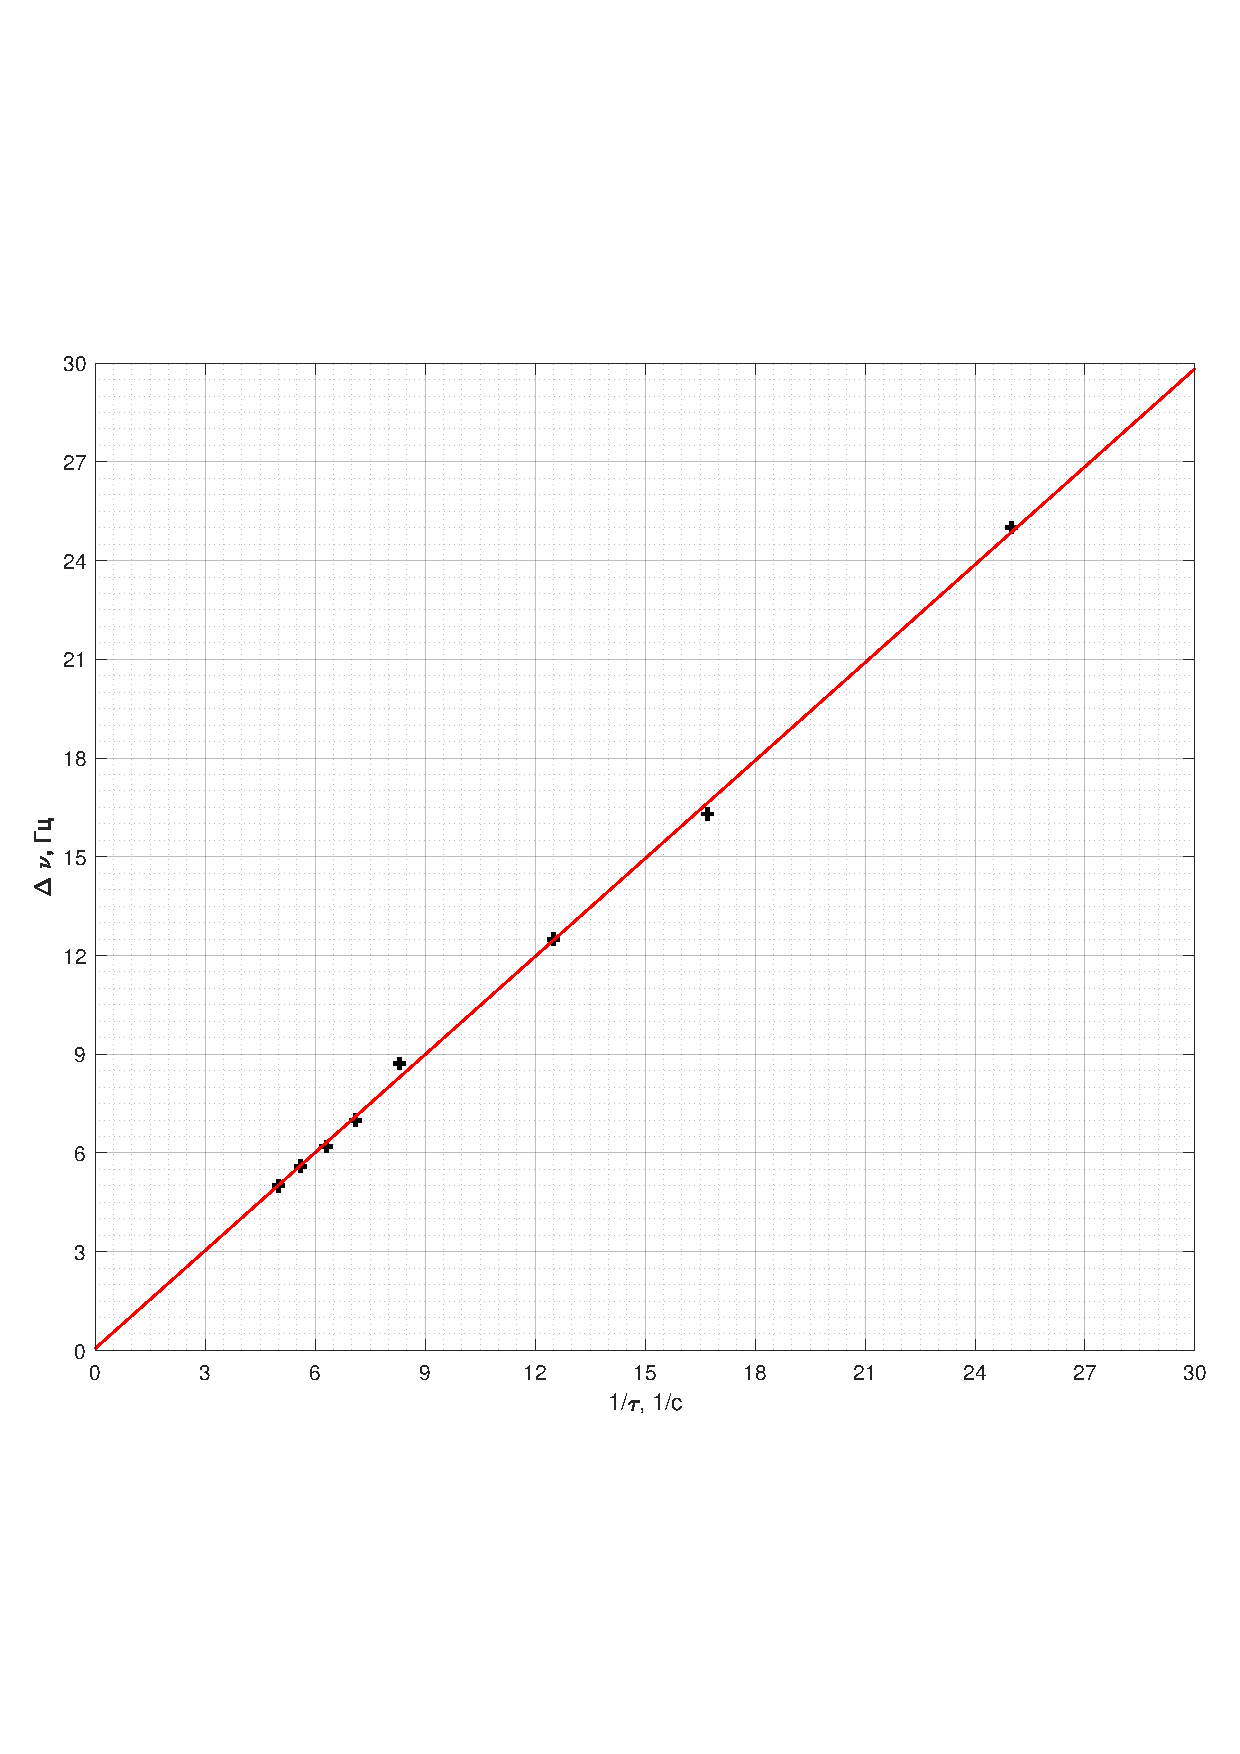
\includegraphics[width=\linewidth]{gr1.pdf}
		\caption{График зависимости периода решетки, взятого по спектру, от диаметра диафрагмы $d(1/D_{min})$}
		\label{oops}
	\end{figure}
\end{center}

\section*{Наблюдение пространственной фильтрации}

В этой части работы будем работать с решеткой №2.

Максимумы, создаваемые двумерной решеткой в фокальной плоскости объектива $F$ (см. рисунок \ref{abbe}), представляют картину дифракции Фраунгофера и будут рассмотрены как первичное изображение. Они изображены на рисунке \ref{2d}.

\begin{figure}[h]
	\centering	
	\includegraphics[width=0.3\textwidth]{2d.png}
	\caption{Дифракция Фраунгофера на двумерной решетке}
	\label{2d}
\end{figure}

Отфильтруем максимумы в одном из направлений решетки. Для этого подберем ширину щели таким образом, чтобы она пропускала только максимум нулевого порядка в перпендикулярном направлении. Поворачивая щель относительно оси системы, пронаблюдаем, как изменяется картина на экране, демонстрируя пространственную фильтрацию. 

При вертикальной щели пропускаются максимумы $(0, m_x)$, и на экране наблюдается вертикальная "полоса" \ размытых максимумов. При горизонтальной щели, наоборот, пропускаются максимумы $(m_y, 0)$, и на экране видна горизонтальная "полоса". При положении щели под углом $45^\circ$ к вертикали наблюдается полоса максимумов $m_x = m_y$. Фотографии эффекта приведены на рисунке \ref{rotate}. 

\begin{figure}[h]
	\begin{minipage}[h]{0.3\linewidth}
		\center{\includegraphics[width=0.9\linewidth]{vert.jpg} \\ a)}
	\end{minipage}
	\hfill
	\begin{minipage}[h]{0.3\linewidth}
		\center{\includegraphics[width=0.9\linewidth]{mid.jpg} \\ b)}
	\end{minipage}
	\hfill
	\begin{minipage}[h]{0.3\linewidth}
		\center{\includegraphics[width=0.9\linewidth]{hor.jpg} \\ c)}
	\end{minipage}
	\caption{Наблюдаемая картинка пространственной фильтрации: (a) при вертикальной щели, (b) при наклонной на $45^\circ$ щели, (c) горизонтальной щели }
	\label{rotate}
\end{figure}




\section*{Вывод} 

В работе определены периоды исследуемых решеток тремя методами: по пространственному спектру, по увеличенному микроскопом изображению и по оценке разрешающей способности микроскопа (указаны в таблицах \ref{period1}-\ref{period3}). Полученные значения изменяются в пределах 20\%. Более достоверными являются измерения в первой части работы (по спектру), так как они в меньшей степени зависят от качества установки и настройки системы. 

Проверена теория Аббе разрешающей способности микроскопа, для чего построен график зависимости $d(1/D_{min})$, теоретически являющейся линейной. Действительно, экспериментальные точки хорошо легли на прямую, и коэффициент ее наклона, определенный по графику $b_{exp} = (0.108 \pm 0.012) \text{ мм}^2$ соотносится с теоретической константой $b_{theor} \approx 0.117$, что подтверждает состоятельность метода Аббе.

Изучены эффекты пространственной фильтрации.  

\end{document}